\documentclass[1p]{elsarticle_modified}
%\bibliographystyle{elsarticle-num}

%\usepackage[colorlinks]{hyperref}
%\usepackage{abbrmath_seonhwa} %\Abb, \Ascr, \Acal ,\Abf, \Afrak
\usepackage{amsfonts}
\usepackage{amssymb}
\usepackage{amsmath}
\usepackage{amsthm}
\usepackage{scalefnt}
\usepackage{amsbsy}
\usepackage{kotex}
\usepackage{caption}
\usepackage{subfig}
\usepackage{color}
\usepackage{graphicx}
\usepackage{xcolor} %% white, black, red, green, blue, cyan, magenta, yellow
\usepackage{float}
\usepackage{setspace}
\usepackage{hyperref}

\usepackage{tikz}
\usetikzlibrary{arrows}

\usepackage{multirow}
\usepackage{array} % fixed length table
\usepackage{hhline}

%%%%%%%%%%%%%%%%%%%%%
\makeatletter
\renewcommand*\env@matrix[1][\arraystretch]{%
	\edef\arraystretch{#1}%
	\hskip -\arraycolsep
	\let\@ifnextchar\new@ifnextchar
	\array{*\c@MaxMatrixCols c}}
\makeatother %https://tex.stackexchange.com/questions/14071/how-can-i-increase-the-line-spacing-in-a-matrix
%%%%%%%%%%%%%%%

\usepackage[normalem]{ulem}

\newcommand{\msout}[1]{\ifmmode\text{\sout{\ensuremath{#1}}}\else\sout{#1}\fi}
%SOURCE: \msout is \stkout macro in https://tex.stackexchange.com/questions/20609/strikeout-in-math-mode

\newcommand{\cancel}[1]{
	\ifmmode
	{\color{red}\msout{#1}}
	\else
	{\color{red}\sout{#1}}
	\fi
}

\newcommand{\add}[1]{
	{\color{blue}\uwave{#1}}
}

\newcommand{\replace}[2]{
	\ifmmode
	{\color{red}\msout{#1}}{\color{blue}\uwave{#2}}
	\else
	{\color{red}\sout{#1}}{\color{blue}\uwave{#2}}
	\fi
}

\newcommand{\Sol}{\mathcal{S}} %segment
\newcommand{\D}{D} %diagram
\newcommand{\A}{\mathcal{A}} %arc


%%%%%%%%%%%%%%%%%%%%%%%%%%%%%5 test

\def\sl{\operatorname{\textup{SL}}(2,\Cbb)}
\def\psl{\operatorname{\textup{PSL}}(2,\Cbb)}
\def\quan{\mkern 1mu \triangleright \mkern 1mu}

\theoremstyle{definition}
\newtheorem{thm}{Theorem}[section]
\newtheorem{prop}[thm]{Proposition}
\newtheorem{lem}[thm]{Lemma}
\newtheorem{ques}[thm]{Question}
\newtheorem{cor}[thm]{Corollary}
\newtheorem{defn}[thm]{Definition}
\newtheorem{exam}[thm]{Example}
\newtheorem{rmk}[thm]{Remark}
\newtheorem{alg}[thm]{Algorithm}

\newcommand{\I}{\sqrt{-1}}
\begin{document}

%\begin{frontmatter}
%
%\title{Boundary parabolic representations of knots up to 8 crossings}
%
%%% Group authors per affiliation:
%\author{Yunhi Cho} 
%\address{Department of Mathematics, University of Seoul, Seoul, Korea}
%\ead{yhcho@uos.ac.kr}
%
%
%\author{Seonhwa Kim} %\fnref{s_kim}}
%\address{Center for Geometry and Physics, Institute for Basic Science, Pohang, 37673, Korea}
%\ead{ryeona17@ibs.re.kr}
%
%\author{Hyuk Kim}
%\address{Department of Mathematical Sciences, Seoul National University, Seoul 08826, Korea}
%\ead{hyukkim@snu.ac.kr}
%
%\author{Seokbeom Yoon}
%\address{Department of Mathematical Sciences, Seoul National University, Seoul, 08826,  Korea}
%\ead{sbyoon15@snu.ac.kr}
%
%\begin{abstract}
%We find all boundary parabolic representation of knots up to 8 crossings.
%
%\end{abstract}
%\begin{keyword}
%    \MSC[2010] 57M25 
%\end{keyword}
%
%\end{frontmatter}

%\linenumbers
%\tableofcontents
%
\newcommand\colored[1]{\textcolor{white}{\rule[-0.35ex]{0.8em}{1.4ex}}\kern-0.8em\color{red} #1}%
%\newcommand\colored[1]{\textcolor{white}{ #1}\kern-2.17ex	\textcolor{white}{ #1}\kern-1.81ex	\textcolor{white}{ #1}\kern-2.15ex\color{red}#1	}

{\Large $\underline{12n_{0797}~(K12n_{0797})}$}

\setlength{\tabcolsep}{10pt}
\renewcommand{\arraystretch}{1.6}
\vspace{1cm}\begin{tabular}{m{100pt}>{\centering\arraybackslash}m{274pt}}
\multirow{5}{120pt}{
	\centering
	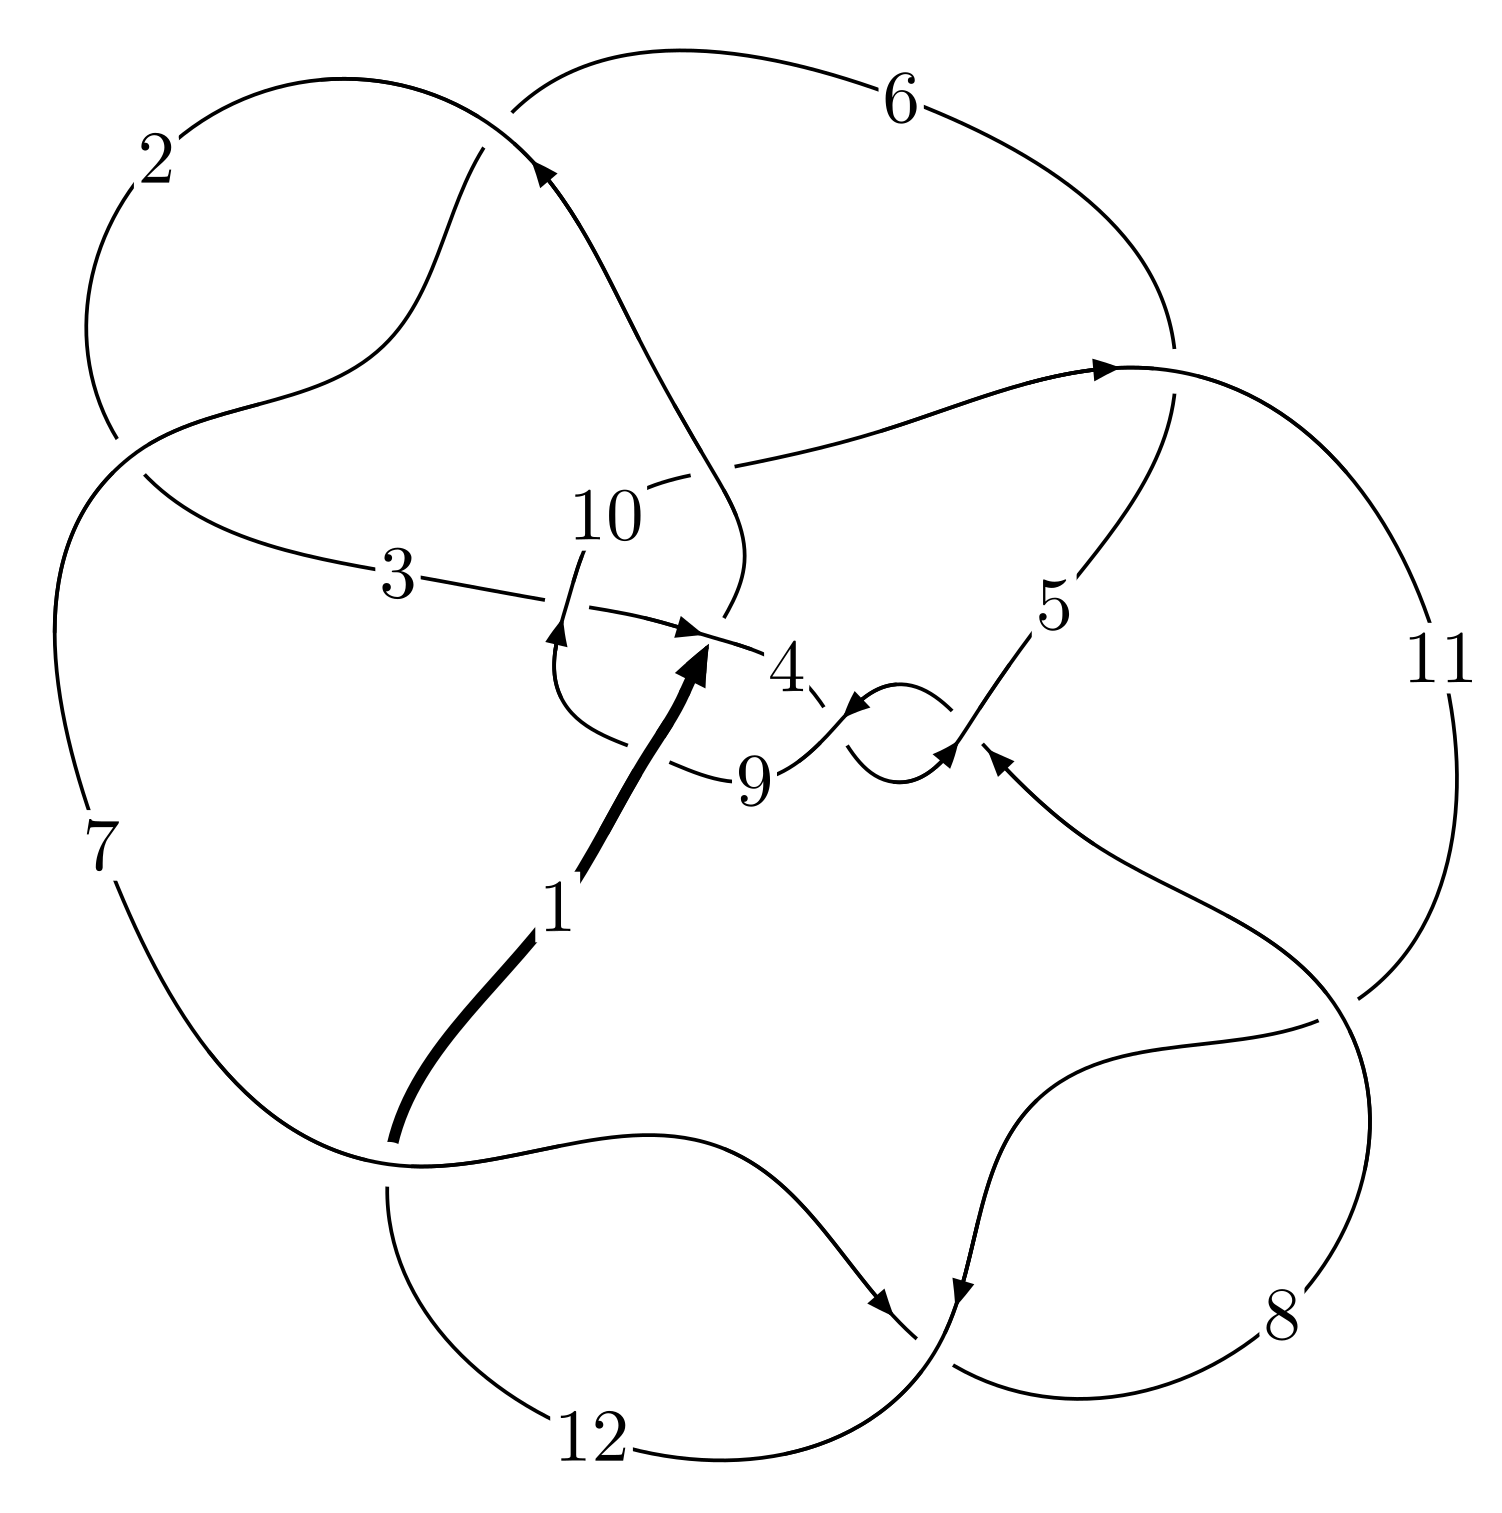
\includegraphics[width=112pt]{../../../GIT/diagram.site/Diagrams/png/2886_12n_0797.png}\\
\ \ \ A knot diagram\footnotemark}&
\allowdisplaybreaks
\textbf{Linearized knot diagam} \\
\cline{2-2}
 &
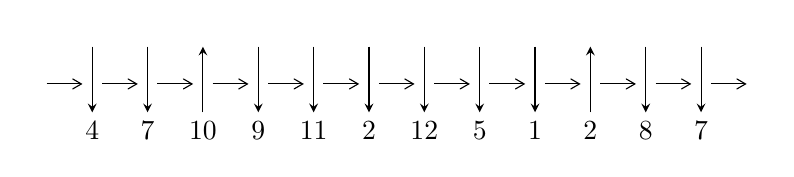
\begin{tikzpicture}[x=20pt, y=17pt]
	% nodes
	\node (C0) at (0, 0) {};
	\node (C1) at (1, 0) {};
	\node (C1U) at (1, +1) {};
	\node (C1D) at (1, -1) {4};

	\node (C2) at (2, 0) {};
	\node (C2U) at (2, +1) {};
	\node (C2D) at (2, -1) {7};

	\node (C3) at (3, 0) {};
	\node (C3U) at (3, +1) {};
	\node (C3D) at (3, -1) {10};

	\node (C4) at (4, 0) {};
	\node (C4U) at (4, +1) {};
	\node (C4D) at (4, -1) {9};

	\node (C5) at (5, 0) {};
	\node (C5U) at (5, +1) {};
	\node (C5D) at (5, -1) {11};

	\node (C6) at (6, 0) {};
	\node (C6U) at (6, +1) {};
	\node (C6D) at (6, -1) {2};

	\node (C7) at (7, 0) {};
	\node (C7U) at (7, +1) {};
	\node (C7D) at (7, -1) {12};

	\node (C8) at (8, 0) {};
	\node (C8U) at (8, +1) {};
	\node (C8D) at (8, -1) {5};

	\node (C9) at (9, 0) {};
	\node (C9U) at (9, +1) {};
	\node (C9D) at (9, -1) {1};

	\node (C10) at (10, 0) {};
	\node (C10U) at (10, +1) {};
	\node (C10D) at (10, -1) {2};

	\node (C11) at (11, 0) {};
	\node (C11U) at (11, +1) {};
	\node (C11D) at (11, -1) {8};

	\node (C12) at (12, 0) {};
	\node (C12U) at (12, +1) {};
	\node (C12D) at (12, -1) {7};
	\node (C13) at (13, 0) {};

	% arrows
	\draw[->,>={angle 60}]
	(C0) edge (C1) (C1) edge (C2) (C2) edge (C3) (C3) edge (C4) (C4) edge (C5) (C5) edge (C6) (C6) edge (C7) (C7) edge (C8) (C8) edge (C9) (C9) edge (C10) (C10) edge (C11) (C11) edge (C12) (C12) edge (C13) ;	\draw[->,>=stealth]
	(C1U) edge (C1D) (C2U) edge (C2D) (C3D) edge (C3U) (C4U) edge (C4D) (C5U) edge (C5D) (C6U) edge (C6D) (C7U) edge (C7D) (C8U) edge (C8D) (C9U) edge (C9D) (C10D) edge (C10U) (C11U) edge (C11D) (C12U) edge (C12D) ;
	\end{tikzpicture} \\
\hhline{~~} \\& 
\textbf{Solving Sequence} \\ \cline{2-2} 
 &
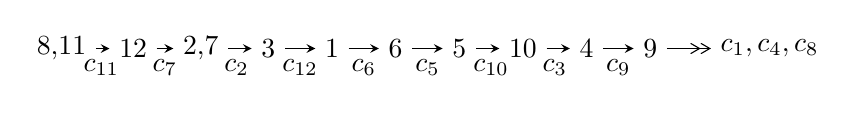
\begin{tikzpicture}[x=23pt, y=7pt]
	% node
	\node (A0) at (-1/8, 0) {8,11};
	\node (A1) at (1, 0) {12};
	\node (A2) at (33/16, 0) {2,7};
	\node (A3) at (25/8, 0) {3};
	\node (A4) at (33/8, 0) {1};
	\node (A5) at (41/8, 0) {6};
	\node (A6) at (49/8, 0) {5};
	\node (A7) at (57/8, 0) {10};
	\node (A8) at (65/8, 0) {4};
	\node (A9) at (73/8, 0) {9};
	\node (C1) at (1/2, -1) {$c_{11}$};
	\node (C2) at (3/2, -1) {$c_{7}$};
	\node (C3) at (21/8, -1) {$c_{2}$};
	\node (C4) at (29/8, -1) {$c_{12}$};
	\node (C5) at (37/8, -1) {$c_{6}$};
	\node (C6) at (45/8, -1) {$c_{5}$};
	\node (C7) at (53/8, -1) {$c_{10}$};
	\node (C8) at (61/8, -1) {$c_{3}$};
	\node (C9) at (69/8, -1) {$c_{9}$};
	\node (A10) at (11, 0) {$c_{1},c_{4},c_{8}$};

	% edge
	\draw[->,>=stealth]	
	(A0) edge (A1) (A1) edge (A2) (A2) edge (A3) (A3) edge (A4) (A4) edge (A5) (A5) edge (A6) (A6) edge (A7) (A7) edge (A8) (A8) edge (A9) ;
	\draw[->>,>={angle 60}]	
	(A9) edge (A10);
\end{tikzpicture} \\ 

\end{tabular} \\

\footnotetext{
The image of knot diagram is generated by the software ``\textbf{Draw programme}" developed by Andrew Bartholomew(\url{http://www.layer8.co.uk/maths/draw/index.htm\#Running-draw}), where we modified some parts for our purpose(\url{https://github.com/CATsTAILs/LinksPainter}).
}\phantom \\ \newline 
\centering \textbf{Ideals for irreducible components\footnotemark of $X_{\text{par}}$} 
 
\begin{align*}
I^u_{1}&=\langle 
2.07960\times10^{91} u^{54}+2.94820\times10^{91} u^{53}+\cdots+1.60845\times10^{93} b-8.75300\times10^{93},\\
\phantom{I^u_{1}}&\phantom{= \langle  }3.49565\times10^{93} u^{54}+1.25650\times10^{94} u^{53}+\cdots+2.58961\times10^{95} a+8.81973\times10^{95},\\
\phantom{I^u_{1}}&\phantom{= \langle  }u^{55}+2 u^{54}+\cdots+547 u+161\rangle \\
I^u_{2}&=\langle 
2 u^{25}-88 u^{24}+\cdots+46 b-59,\;-91 u^{25}+215 u^{24}+\cdots+46 a+66,\;u^{26}- u^{25}+\cdots+4 u+1\rangle \\
\\
\end{align*}
\raggedright * 2 irreducible components of $\dim_{\mathbb{C}}=0$, with total 81 representations.\\
\footnotetext{All coefficients of polynomials are rational numbers. But the coefficients are sometimes approximated in decimal forms when there is not enough margin.}
\newpage
\renewcommand{\arraystretch}{1}
\centering \section*{I. $I^u_{1}= \langle 2.08\times10^{91} u^{54}+2.95\times10^{91} u^{53}+\cdots+1.61\times10^{93} b-8.75\times10^{93},\;3.50\times10^{93} u^{54}+1.26\times10^{94} u^{53}+\cdots+2.59\times10^{95} a+8.82\times10^{95},\;u^{55}+2 u^{54}+\cdots+547 u+161 \rangle$}
\flushleft \textbf{(i) Arc colorings}\\
\begin{tabular}{m{7pt} m{180pt} m{7pt} m{180pt} }
\flushright $a_{8}=$&$\begin{pmatrix}0\\u\end{pmatrix}$ \\
\flushright $a_{11}=$&$\begin{pmatrix}1\\0\end{pmatrix}$ \\
\flushright $a_{12}=$&$\begin{pmatrix}1\\u^2\end{pmatrix}$ \\
\flushright $a_{2}=$&$\begin{pmatrix}-0.0134987 u^{54}-0.0485208 u^{53}+\cdots-12.9886 u-3.40581\\-0.0129292 u^{54}-0.0183294 u^{53}+\cdots+18.5763 u+5.44188\end{pmatrix}$ \\
\flushright $a_{7}=$&$\begin{pmatrix}u\\u^3+u\end{pmatrix}$ \\
\flushright $a_{3}=$&$\begin{pmatrix}-0.0187035 u^{54}-0.0547457 u^{53}+\cdots-3.27141 u-0.392712\\-0.0151382 u^{54}-0.0181689 u^{53}+\cdots+26.8425 u+7.78127\end{pmatrix}$ \\
\flushright $a_{1}=$&$\begin{pmatrix}u^2+1\\u^4+2 u^2\end{pmatrix}$ \\
\flushright $a_{6}=$&$\begin{pmatrix}-0.0211190 u^{54}-0.0418297 u^{53}+\cdots-8.19248 u+0.487545\\0.0160121 u^{54}+0.0367680 u^{53}+\cdots+6.73323 u-0.603776\end{pmatrix}$ \\
\flushright $a_{5}=$&$\begin{pmatrix}-0.00510696 u^{54}-0.00506179 u^{53}+\cdots-1.45925 u-0.116231\\0.0160121 u^{54}+0.0367680 u^{53}+\cdots+6.73323 u-0.603776\end{pmatrix}$ \\
\flushright $a_{10}=$&$\begin{pmatrix}0.0168284 u^{54}+0.0417284 u^{53}+\cdots+17.8209 u+3.35274\\0.0107121 u^{54}+0.00850273 u^{53}+\cdots-25.3078 u-6.73136\end{pmatrix}$ \\
\flushright $a_{4}=$&$\begin{pmatrix}0.00524703 u^{54}+0.0251477 u^{53}+\cdots+38.4021 u+9.27761\\0.0246750 u^{54}+0.0506644 u^{53}+\cdots-1.69128 u-1.40430\end{pmatrix}$ \\
\flushright $a_{9}=$&$\begin{pmatrix}0.0213925 u^{54}+0.0472947 u^{53}+\cdots+8.93888 u+0.875826\\0.00408564 u^{54}-0.00772075 u^{53}+\cdots-24.1554 u-5.78092\end{pmatrix}$\\&\end{tabular}
\flushleft \textbf{(ii) Obstruction class $= -1$}\\~\\
\flushleft \textbf{(iii) Cusp Shapes $= -0.0784770 u^{54}-0.193082 u^{53}+\cdots-68.0047 u-10.6801$}\\~\\
\newpage\renewcommand{\arraystretch}{1}
\flushleft \textbf{(iv) u-Polynomials at the component}\newline \\
\begin{tabular}{m{50pt}|m{274pt}}
Crossings & \hspace{64pt}u-Polynomials at each crossing \\
\hline $$\begin{aligned}c_{1}\end{aligned}$$&$\begin{aligned}
&u^{55}-6 u^{54}+\cdots+138 u-7
\end{aligned}$\\
\hline $$\begin{aligned}c_{2},c_{6}\end{aligned}$$&$\begin{aligned}
&u^{55}- u^{54}+\cdots-6215 u+4261
\end{aligned}$\\
\hline $$\begin{aligned}c_{3}\end{aligned}$$&$\begin{aligned}
&u^{55}-22 u^{53}+\cdots-425241 u+68743
\end{aligned}$\\
\hline $$\begin{aligned}c_{4},c_{8}\end{aligned}$$&$\begin{aligned}
&u^{55}+3 u^{54}+\cdots+40 u+8
\end{aligned}$\\
\hline $$\begin{aligned}c_{5}\end{aligned}$$&$\begin{aligned}
&u^{55}+u^{54}+\cdots+518 u+691
\end{aligned}$\\
\hline $$\begin{aligned}c_{7},c_{11},c_{12}\end{aligned}$$&$\begin{aligned}
&u^{55}+2 u^{54}+\cdots+547 u+161
\end{aligned}$\\
\hline $$\begin{aligned}c_{9}\end{aligned}$$&$\begin{aligned}
&u^{55}+6 u^{54}+\cdots+3961 u+547
\end{aligned}$\\
\hline $$\begin{aligned}c_{10}\end{aligned}$$&$\begin{aligned}
&u^{55}-45 u^{53}+\cdots+42944 u+11864
\end{aligned}$\\
\hline
\end{tabular}\\~\\
\newpage\renewcommand{\arraystretch}{1}
\flushleft \textbf{(v) Riley Polynomials at the component}\newline \\
\begin{tabular}{m{50pt}|m{274pt}}
Crossings & \hspace{64pt}Riley Polynomials at each crossing \\
\hline $$\begin{aligned}c_{1}\end{aligned}$$&$\begin{aligned}
&y^{55}+10 y^{54}+\cdots+9314 y-49
\end{aligned}$\\
\hline $$\begin{aligned}c_{2},c_{6}\end{aligned}$$&$\begin{aligned}
&y^{55}+81 y^{54}+\cdots-714727097 y-18156121
\end{aligned}$\\
\hline $$\begin{aligned}c_{3}\end{aligned}$$&$\begin{aligned}
&y^{55}-44 y^{54}+\cdots+161699281125 y-4725600049
\end{aligned}$\\
\hline $$\begin{aligned}c_{4},c_{8}\end{aligned}$$&$\begin{aligned}
&y^{55}+51 y^{54}+\cdots-16448 y-64
\end{aligned}$\\
\hline $$\begin{aligned}c_{5}\end{aligned}$$&$\begin{aligned}
&y^{55}+83 y^{54}+\cdots-17632722 y-477481
\end{aligned}$\\
\hline $$\begin{aligned}c_{7},c_{11},c_{12}\end{aligned}$$&$\begin{aligned}
&y^{55}+68 y^{54}+\cdots-615593 y-25921
\end{aligned}$\\
\hline $$\begin{aligned}c_{9}\end{aligned}$$&$\begin{aligned}
&y^{55}+24 y^{54}+\cdots-5301057 y-299209
\end{aligned}$\\
\hline $$\begin{aligned}c_{10}\end{aligned}$$&$\begin{aligned}
&y^{55}-90 y^{54}+\cdots+3812472192 y-140754496
\end{aligned}$\\
\hline
\end{tabular}\\~\\
\newpage\flushleft \textbf{(vi) Complex Volumes and Cusp Shapes}
$$\begin{array}{c|c|c}  
\text{Solutions to }I^u_{1}& \I (\text{vol} + \sqrt{-1}CS) & \text{Cusp shape}\\
 \hline 
\begin{aligned}
u &= \phantom{-}0.490040 + 0.753457 I \\
a &= -0.887738 - 0.559278 I \\
b &= \phantom{-}1.50685 - 0.03038 I\end{aligned}
 & \phantom{-}6.13669 - 4.64981 I & -5.28628 + 6.18804 I \\ \hline\begin{aligned}
u &= \phantom{-}0.490040 - 0.753457 I \\
a &= -0.887738 + 0.559278 I \\
b &= \phantom{-}1.50685 + 0.03038 I\end{aligned}
 & \phantom{-}6.13669 + 4.64981 I & -5.28628 - 6.18804 I \\ \hline\begin{aligned}
u &= \phantom{-}0.570071 + 0.997038 I \\
a &= \phantom{-}0.88532 + 1.33081 I \\
b &= -0.537901 + 0.521935 I\end{aligned}
 & -1.18456 - 2.16066 I & \phantom{-0.000000 } 0 \\ \hline\begin{aligned}
u &= \phantom{-}0.570071 - 0.997038 I \\
a &= \phantom{-}0.88532 - 1.33081 I \\
b &= -0.537901 - 0.521935 I\end{aligned}
 & -1.18456 + 2.16066 I & \phantom{-0.000000 } 0 \\ \hline\begin{aligned}
u &= \phantom{-}0.251956 + 0.785395 I \\
a &= -1.08299 - 1.33546 I \\
b &= \phantom{-}1.61042 - 0.04562 I\end{aligned}
 & \phantom{-}9.54903 - 0.14815 I & \phantom{-}1.97076 + 0.45693 I \\ \hline\begin{aligned}
u &= \phantom{-}0.251956 - 0.785395 I \\
a &= -1.08299 + 1.33546 I \\
b &= \phantom{-}1.61042 + 0.04562 I\end{aligned}
 & \phantom{-}9.54903 + 0.14815 I & \phantom{-}1.97076 - 0.45693 I \\ \hline\begin{aligned}
u &= -0.116882 + 1.178060 I \\
a &= \phantom{-}0.104386 - 0.227431 I \\
b &= -0.646640 - 0.042880 I\end{aligned}
 & \phantom{-}2.57075 + 2.07006 I & \phantom{-0.000000 } 0 \\ \hline\begin{aligned}
u &= -0.116882 - 1.178060 I \\
a &= \phantom{-}0.104386 + 0.227431 I \\
b &= -0.646640 + 0.042880 I\end{aligned}
 & \phantom{-}2.57075 - 2.07006 I & \phantom{-0.000000 } 0 \\ \hline\begin{aligned}
u &= -0.636334 + 1.002860 I \\
a &= \phantom{-}0.811613 - 0.985736 I \\
b &= -0.254278 - 1.303390 I\end{aligned}
 & -0.34669 + 2.38010 I & \phantom{-0.000000 } 0 \\ \hline\begin{aligned}
u &= -0.636334 - 1.002860 I \\
a &= \phantom{-}0.811613 + 0.985736 I \\
b &= -0.254278 + 1.303390 I\end{aligned}
 & -0.34669 - 2.38010 I & \phantom{-0.000000 } 0\\
 \hline 
 \end{array}$$\newpage$$\begin{array}{c|c|c}  
\text{Solutions to }I^u_{1}& \I (\text{vol} + \sqrt{-1}CS) & \text{Cusp shape}\\
 \hline 
\begin{aligned}
u &= \phantom{-}0.516300 + 0.607161 I \\
a &= \phantom{-}0.551523 + 0.748786 I \\
b &= -1.57349 - 0.23422 I\end{aligned}
 & \phantom{-}5.55349 + 1.15098 I & -7.02981 + 2.01750 I \\ \hline\begin{aligned}
u &= \phantom{-}0.516300 - 0.607161 I \\
a &= \phantom{-}0.551523 - 0.748786 I \\
b &= -1.57349 + 0.23422 I\end{aligned}
 & \phantom{-}5.55349 - 1.15098 I & -7.02981 - 2.01750 I \\ \hline\begin{aligned}
u &= \phantom{-}0.635640 + 0.408514 I \\
a &= -0.049474 - 0.375979 I \\
b &= \phantom{-}0.244897 + 0.404452 I\end{aligned}
 & \phantom{-}3.21037 - 3.81410 I & -3.00876 + 4.44084 I \\ \hline\begin{aligned}
u &= \phantom{-}0.635640 - 0.408514 I \\
a &= -0.049474 + 0.375979 I \\
b &= \phantom{-}0.244897 - 0.404452 I\end{aligned}
 & \phantom{-}3.21037 + 3.81410 I & -3.00876 - 4.44084 I \\ \hline\begin{aligned}
u &= \phantom{-}0.578207 + 0.479856 I \\
a &= \phantom{-}0.433436 + 0.026732 I \\
b &= -0.483722 + 0.114833 I\end{aligned}
 & \phantom{-}3.53350 - 0.19360 I & -3.73389 + 2.78818 I \\ \hline\begin{aligned}
u &= \phantom{-}0.578207 - 0.479856 I \\
a &= \phantom{-}0.433436 - 0.026732 I \\
b &= -0.483722 - 0.114833 I\end{aligned}
 & \phantom{-}3.53350 + 0.19360 I & -3.73389 - 2.78818 I \\ \hline\begin{aligned}
u &= \phantom{-}0.084715 + 0.743739 I \\
a &= -0.86276 - 2.38888 I \\
b &= \phantom{-}0.302921 + 0.216438 I\end{aligned}
 & \phantom{-}1.83611 + 5.00955 I & -1.41995 - 4.51640 I \\ \hline\begin{aligned}
u &= \phantom{-}0.084715 - 0.743739 I \\
a &= -0.86276 + 2.38888 I \\
b &= \phantom{-}0.302921 - 0.216438 I\end{aligned}
 & \phantom{-}1.83611 - 5.00955 I & -1.41995 + 4.51640 I \\ \hline\begin{aligned}
u &= -0.206657 + 0.671508 I \\
a &= -0.30812 + 1.43958 I \\
b &= -0.371827 + 1.206250 I\end{aligned}
 & \phantom{-}1.53161 - 4.54582 I & -1.70666 + 0.80391 I \\ \hline\begin{aligned}
u &= -0.206657 - 0.671508 I \\
a &= -0.30812 - 1.43958 I \\
b &= -0.371827 - 1.206250 I\end{aligned}
 & \phantom{-}1.53161 + 4.54582 I & -1.70666 - 0.80391 I\\
 \hline 
 \end{array}$$\newpage$$\begin{array}{c|c|c}  
\text{Solutions to }I^u_{1}& \I (\text{vol} + \sqrt{-1}CS) & \text{Cusp shape}\\
 \hline 
\begin{aligned}
u &= \phantom{-}0.223556 + 0.606477 I \\
a &= \phantom{-}0.602584 + 1.250130 I \\
b &= -1.89077 + 0.29080 I\end{aligned}
 & \phantom{-}8.94290 - 1.49383 I & \phantom{-}1.30346 + 4.21129 I \\ \hline\begin{aligned}
u &= \phantom{-}0.223556 - 0.606477 I \\
a &= \phantom{-}0.602584 - 1.250130 I \\
b &= -1.89077 - 0.29080 I\end{aligned}
 & \phantom{-}8.94290 + 1.49383 I & \phantom{-}1.30346 - 4.21129 I \\ \hline\begin{aligned}
u &= -1.116550 + 0.829939 I \\
a &= -0.054400 + 0.756088 I \\
b &= \phantom{-}2.34708 + 0.06527 I\end{aligned}
 & \phantom{-}12.4197 + 8.7555 I & \phantom{-0.000000 } 0 \\ \hline\begin{aligned}
u &= -1.116550 - 0.829939 I \\
a &= -0.054400 - 0.756088 I \\
b &= \phantom{-}2.34708 - 0.06527 I\end{aligned}
 & \phantom{-}12.4197 - 8.7555 I & \phantom{-0.000000 } 0 \\ \hline\begin{aligned}
u &= -0.129598 + 1.407450 I \\
a &= -0.933650 - 0.404509 I \\
b &= \phantom{-}0.363613 + 1.022520 I\end{aligned}
 & \phantom{-}4.96026 + 2.94833 I & \phantom{-0.000000 } 0 \\ \hline\begin{aligned}
u &= -0.129598 - 1.407450 I \\
a &= -0.933650 + 0.404509 I \\
b &= \phantom{-}0.363613 - 1.022520 I\end{aligned}
 & \phantom{-}4.96026 - 2.94833 I & \phantom{-0.000000 } 0 \\ \hline\begin{aligned}
u &= -1.29784 + 0.63122 I \\
a &= -0.058295 - 0.824045 I \\
b &= -2.36846 - 0.46156 I\end{aligned}
 & \phantom{-}11.71150 - 0.95890 I & \phantom{-0.000000 } 0 \\ \hline\begin{aligned}
u &= -1.29784 - 0.63122 I \\
a &= -0.058295 + 0.824045 I \\
b &= -2.36846 + 0.46156 I\end{aligned}
 & \phantom{-}11.71150 + 0.95890 I & \phantom{-0.000000 } 0 \\ \hline\begin{aligned}
u &= -0.18355 + 1.46859 I \\
a &= \phantom{-}0.384347 - 0.500239 I \\
b &= -0.278834 - 0.427014 I\end{aligned}
 & \phantom{-}4.72513 + 1.63928 I & \phantom{-0.000000 } 0 \\ \hline\begin{aligned}
u &= -0.18355 - 1.46859 I \\
a &= \phantom{-}0.384347 + 0.500239 I \\
b &= -0.278834 + 0.427014 I\end{aligned}
 & \phantom{-}4.72513 - 1.63928 I & \phantom{-0.000000 } 0\\
 \hline 
 \end{array}$$\newpage$$\begin{array}{c|c|c}  
\text{Solutions to }I^u_{1}& \I (\text{vol} + \sqrt{-1}CS) & \text{Cusp shape}\\
 \hline 
\begin{aligned}
u &= \phantom{-}0.22442 + 1.46665 I \\
a &= -0.758599 - 0.218438 I \\
b &= \phantom{-}0.711269 + 0.025399 I\end{aligned}
 & \phantom{-}9.77580 - 3.16441 I & \phantom{-0.000000 } 0 \\ \hline\begin{aligned}
u &= \phantom{-}0.22442 - 1.46665 I \\
a &= -0.758599 + 0.218438 I \\
b &= \phantom{-}0.711269 - 0.025399 I\end{aligned}
 & \phantom{-}9.77580 + 3.16441 I & \phantom{-0.000000 } 0 \\ \hline\begin{aligned}
u &= \phantom{-}0.22595 + 1.46861 I \\
a &= \phantom{-}0.078711 + 0.724552 I \\
b &= -0.246015 - 0.635654 I\end{aligned}
 & \phantom{-}9.28337 - 6.93920 I & \phantom{-0.000000 } 0 \\ \hline\begin{aligned}
u &= \phantom{-}0.22595 - 1.46861 I \\
a &= \phantom{-}0.078711 - 0.724552 I \\
b &= -0.246015 + 0.635654 I\end{aligned}
 & \phantom{-}9.28337 + 6.93920 I & \phantom{-0.000000 } 0 \\ \hline\begin{aligned}
u &= -0.295289 + 0.365913 I \\
a &= \phantom{-}0.546011 - 1.002610 I \\
b &= -0.236263 - 0.861145 I\end{aligned}
 & -0.63078 + 1.39813 I & -4.91291 - 6.55485 I \\ \hline\begin{aligned}
u &= -0.295289 - 0.365913 I \\
a &= \phantom{-}0.546011 + 1.002610 I \\
b &= -0.236263 + 0.861145 I\end{aligned}
 & -0.63078 - 1.39813 I & -4.91291 + 6.55485 I \\ \hline\begin{aligned}
u &= -0.426697\phantom{ +0.000000I} \\
a &= \phantom{-}1.04155\phantom{ +0.000000I} \\
b &= \phantom{-}0.354185\phantom{ +0.000000I}\end{aligned}
 & -0.877261\phantom{ +0.000000I} & -10.1120\phantom{ +0.000000I} \\ \hline\begin{aligned}
u &= \phantom{-}0.06992 + 1.64735 I \\
a &= -2.21340 + 0.12521 I \\
b &= \phantom{-}2.70602 - 0.87673 I\end{aligned}
 & \phantom{-}17.0119 - 2.6386 I & \phantom{-0.000000 } 0 \\ \hline\begin{aligned}
u &= \phantom{-}0.06992 - 1.64735 I \\
a &= -2.21340 - 0.12521 I \\
b &= \phantom{-}2.70602 + 0.87673 I\end{aligned}
 & \phantom{-}17.0119 + 2.6386 I & \phantom{-0.000000 } 0 \\ \hline\begin{aligned}
u &= \phantom{-}0.14782 + 1.66795 I \\
a &= -1.88593 - 0.44797 I \\
b &= \phantom{-}2.33419 - 0.02631 I\end{aligned}
 & \phantom{-}13.66400 - 1.40536 I & \phantom{-0.000000 } 0\\
 \hline 
 \end{array}$$\newpage$$\begin{array}{c|c|c}  
\text{Solutions to }I^u_{1}& \I (\text{vol} + \sqrt{-1}CS) & \text{Cusp shape}\\
 \hline 
\begin{aligned}
u &= \phantom{-}0.14782 - 1.66795 I \\
a &= -1.88593 + 0.44797 I \\
b &= \phantom{-}2.33419 + 0.02631 I\end{aligned}
 & \phantom{-}13.66400 + 1.40536 I & \phantom{-0.000000 } 0 \\ \hline\begin{aligned}
u &= -0.194738 + 0.240755 I \\
a &= \phantom{-}1.82364 + 2.49499 I \\
b &= \phantom{-}0.421348 - 0.103727 I\end{aligned}
 & -1.054960 - 0.149529 I & -3.90095 - 3.89450 I \\ \hline\begin{aligned}
u &= -0.194738 - 0.240755 I \\
a &= \phantom{-}1.82364 - 2.49499 I \\
b &= \phantom{-}0.421348 + 0.103727 I\end{aligned}
 & -1.054960 + 0.149529 I & -3.90095 + 3.89450 I \\ \hline\begin{aligned}
u &= \phantom{-}0.15421 + 1.68561 I \\
a &= \phantom{-}1.84022 + 0.35608 I \\
b &= -2.13772 + 0.11444 I\end{aligned}
 & \phantom{-}14.7179 - 7.2096 I & \phantom{-0.000000 } 0 \\ \hline\begin{aligned}
u &= \phantom{-}0.15421 - 1.68561 I \\
a &= \phantom{-}1.84022 - 0.35608 I \\
b &= -2.13772 - 0.11444 I\end{aligned}
 & \phantom{-}14.7179 + 7.2096 I & \phantom{-0.000000 } 0 \\ \hline\begin{aligned}
u &= \phantom{-}0.08151 + 1.71479 I \\
a &= \phantom{-}1.71136 + 0.13502 I \\
b &= -2.00460 + 0.60101 I\end{aligned}
 & \phantom{-}18.6220 - 1.5785 I & \phantom{-0.000000 } 0 \\ \hline\begin{aligned}
u &= \phantom{-}0.08151 - 1.71479 I \\
a &= \phantom{-}1.71136 - 0.13502 I \\
b &= -2.00460 - 0.60101 I\end{aligned}
 & \phantom{-}18.6220 + 1.5785 I & \phantom{-0.000000 } 0 \\ \hline\begin{aligned}
u &= -0.04620 + 1.72945 I \\
a &= -0.847700 + 0.629686 I \\
b &= \phantom{-}1.26083 - 1.76289 I\end{aligned}
 & \phantom{-}10.49490 - 3.28765 I & \phantom{-0.000000 } 0 \\ \hline\begin{aligned}
u &= -0.04620 - 1.72945 I \\
a &= -0.847700 - 0.629686 I \\
b &= \phantom{-}1.26083 + 1.76289 I\end{aligned}
 & \phantom{-}10.49490 + 3.28765 I & \phantom{-0.000000 } 0 \\ \hline\begin{aligned}
u &= \phantom{-}0.01411 + 1.75354 I \\
a &= \phantom{-}0.705957 - 0.124688 I \\
b &= -0.83820 + 1.26974 I\end{aligned}
 & \phantom{-}11.23260 + 4.25408 I & \phantom{-0.000000 } 0\\
 \hline 
 \end{array}$$\newpage$$\begin{array}{c|c|c}  
\text{Solutions to }I^u_{1}& \I (\text{vol} + \sqrt{-1}CS) & \text{Cusp shape}\\
 \hline 
\begin{aligned}
u &= \phantom{-}0.01411 - 1.75354 I \\
a &= \phantom{-}0.705957 + 0.124688 I \\
b &= -0.83820 - 1.26974 I\end{aligned}
 & \phantom{-}11.23260 - 4.25408 I & \phantom{-0.000000 } 0 \\ \hline\begin{aligned}
u &= -0.36581 + 1.72020 I \\
a &= \phantom{-}1.56485 - 0.63201 I \\
b &= -2.36197 - 0.69629 I\end{aligned}
 & -18.7497 + 14.4065 I & \phantom{-0.000000 } 0 \\ \hline\begin{aligned}
u &= -0.36581 - 1.72020 I \\
a &= \phantom{-}1.56485 + 0.63201 I \\
b &= -2.36197 + 0.69629 I\end{aligned}
 & -18.7497 - 14.4065 I & \phantom{-0.000000 } 0 \\ \hline\begin{aligned}
u &= -0.46563 + 1.76753 I \\
a &= -1.33286 + 0.60148 I \\
b &= \phantom{-}2.24415 + 0.96108 I\end{aligned}
 & \phantom{-}19.3972 + 5.7935 I & \phantom{-0.000000 } 0 \\ \hline\begin{aligned}
u &= -0.46563 - 1.76753 I \\
a &= -1.33286 - 0.60148 I \\
b &= \phantom{-}2.24415 - 0.96108 I\end{aligned}
 & \phantom{-}19.3972 - 5.7935 I & \phantom{-0.000000 } 0\\
 \hline 
 \end{array}$$\newpage\newpage\renewcommand{\arraystretch}{1}
\centering \section*{II. $I^u_{2}= \langle 2 u^{25}-88 u^{24}+\cdots+46 b-59,\;-91 u^{25}+215 u^{24}+\cdots+46 a+66,\;u^{26}- u^{25}+\cdots+4 u+1 \rangle$}
\flushleft \textbf{(i) Arc colorings}\\
\begin{tabular}{m{7pt} m{180pt} m{7pt} m{180pt} }
\flushright $a_{8}=$&$\begin{pmatrix}0\\u\end{pmatrix}$ \\
\flushright $a_{11}=$&$\begin{pmatrix}1\\0\end{pmatrix}$ \\
\flushright $a_{12}=$&$\begin{pmatrix}1\\u^2\end{pmatrix}$ \\
\flushright $a_{2}=$&$\begin{pmatrix}1.97826 u^{25}-4.67391 u^{24}+\cdots+2.36957 u-1.43478\\-0.0434783 u^{25}+1.91304 u^{24}+\cdots+6.47826 u+1.28261\end{pmatrix}$ \\
\flushright $a_{7}=$&$\begin{pmatrix}u\\u^3+u\end{pmatrix}$ \\
\flushright $a_{3}=$&$\begin{pmatrix}3.63043 u^{25}-8.30435 u^{24}+\cdots-1.86957 u-2.76087\\-1.13043 u^{25}+4.67391 u^{24}+\cdots+8.50000 u+1.93478\end{pmatrix}$ \\
\flushright $a_{1}=$&$\begin{pmatrix}u^2+1\\u^4+2 u^2\end{pmatrix}$ \\
\flushright $a_{6}=$&$\begin{pmatrix}-3.23913 u^{25}+2.80435 u^{24}+\cdots-13.1522 u-2.23913\\0.652174 u^{25}+0.434783 u^{24}+\cdots+2.69565 u+0.586957\end{pmatrix}$ \\
\flushright $a_{5}=$&$\begin{pmatrix}-2.58696 u^{25}+3.23913 u^{24}+\cdots-10.4565 u-1.65217\\0.652174 u^{25}+0.434783 u^{24}+\cdots+2.69565 u+0.586957\end{pmatrix}$ \\
\flushright $a_{10}=$&$\begin{pmatrix}0.543478 u^{25}-2.43478 u^{24}+\cdots-4.95652 u-1.58696\\1.52174 u^{25}-1.21739 u^{24}+\cdots+2.52174 u-0.0434783\end{pmatrix}$ \\
\flushright $a_{4}=$&$\begin{pmatrix}-0.717391 u^{25}+0.760870 u^{24}+\cdots+0.195652 u+0.652174\\-1.04348 u^{25}+4.84783 u^{24}+\cdots+7.54348 u+2.36957\end{pmatrix}$ \\
\flushright $a_{9}=$&$\begin{pmatrix}u^{25}-2 u^{24}+\cdots-4 u-2\\1.54348 u^{25}-1.32609 u^{24}+\cdots+1.93478 u-0.0652174\end{pmatrix}$\\&\end{tabular}
\flushleft \textbf{(ii) Obstruction class $= 1$}\\~\\
\flushleft \textbf{(iii) Cusp Shapes $= \frac{55}{23} u^{25}-\frac{266}{23} u^{24}+\cdots+\frac{1}{23} u-\frac{274}{23}$}\\~\\
\newpage\renewcommand{\arraystretch}{1}
\flushleft \textbf{(iv) u-Polynomials at the component}\newline \\
\begin{tabular}{m{50pt}|m{274pt}}
Crossings & \hspace{64pt}u-Polynomials at each crossing \\
\hline $$\begin{aligned}c_{1}\end{aligned}$$&$\begin{aligned}
&u^{26}-9 u^{25}+\cdots-3 u+1
\end{aligned}$\\
\hline $$\begin{aligned}c_{2}\end{aligned}$$&$\begin{aligned}
&u^{26}+7 u^{24}+\cdots-6 u^2+1
\end{aligned}$\\
\hline $$\begin{aligned}c_{3}\end{aligned}$$&$\begin{aligned}
&u^{26}+u^{25}+\cdots+7 u^2+1
\end{aligned}$\\
\hline $$\begin{aligned}c_{4}\end{aligned}$$&$\begin{aligned}
&u^{26}+2 u^{25}+\cdots+8 u+8
\end{aligned}$\\
\hline $$\begin{aligned}c_{5}\end{aligned}$$&$\begin{aligned}
&u^{26}+18 u^{24}+\cdots+155 u+19
\end{aligned}$\\
\hline $$\begin{aligned}c_{6}\end{aligned}$$&$\begin{aligned}
&u^{26}+7 u^{24}+\cdots-6 u^2+1
\end{aligned}$\\
\hline $$\begin{aligned}c_{7}\end{aligned}$$&$\begin{aligned}
&u^{26}+u^{25}+\cdots-4 u+1
\end{aligned}$\\
\hline $$\begin{aligned}c_{8}\end{aligned}$$&$\begin{aligned}
&u^{26}-2 u^{25}+\cdots-8 u+8
\end{aligned}$\\
\hline $$\begin{aligned}c_{9}\end{aligned}$$&$\begin{aligned}
&u^{26}+u^{25}+\cdots-6 u+1
\end{aligned}$\\
\hline $$\begin{aligned}c_{10}\end{aligned}$$&$\begin{aligned}
&u^{26}-3 u^{25}+\cdots-16 u+8
\end{aligned}$\\
\hline $$\begin{aligned}c_{11},c_{12}\end{aligned}$$&$\begin{aligned}
&u^{26}- u^{25}+\cdots+4 u+1
\end{aligned}$\\
\hline
\end{tabular}\\~\\
\newpage\renewcommand{\arraystretch}{1}
\flushleft \textbf{(v) Riley Polynomials at the component}\newline \\
\begin{tabular}{m{50pt}|m{274pt}}
Crossings & \hspace{64pt}Riley Polynomials at each crossing \\
\hline $$\begin{aligned}c_{1}\end{aligned}$$&$\begin{aligned}
&y^{26}- y^{25}+\cdots-3 y+1
\end{aligned}$\\
\hline $$\begin{aligned}c_{2},c_{6}\end{aligned}$$&$\begin{aligned}
&y^{26}+14 y^{25}+\cdots-12 y+1
\end{aligned}$\\
\hline $$\begin{aligned}c_{3}\end{aligned}$$&$\begin{aligned}
&y^{26}-7 y^{25}+\cdots+14 y+1
\end{aligned}$\\
\hline $$\begin{aligned}c_{4},c_{8}\end{aligned}$$&$\begin{aligned}
&y^{26}+20 y^{25}+\cdots+768 y+64
\end{aligned}$\\
\hline $$\begin{aligned}c_{5}\end{aligned}$$&$\begin{aligned}
&y^{26}+36 y^{25}+\cdots-3239 y+361
\end{aligned}$\\
\hline $$\begin{aligned}c_{7},c_{11},c_{12}\end{aligned}$$&$\begin{aligned}
&y^{26}+29 y^{25}+\cdots+8 y+1
\end{aligned}$\\
\hline $$\begin{aligned}c_{9}\end{aligned}$$&$\begin{aligned}
&y^{26}+y^{25}+\cdots+72 y+1
\end{aligned}$\\
\hline $$\begin{aligned}c_{10}\end{aligned}$$&$\begin{aligned}
&y^{26}-17 y^{25}+\cdots+448 y+64
\end{aligned}$\\
\hline
\end{tabular}\\~\\
\newpage\flushleft \textbf{(vi) Complex Volumes and Cusp Shapes}
$$\begin{array}{c|c|c}  
\text{Solutions to }I^u_{2}& \I (\text{vol} + \sqrt{-1}CS) & \text{Cusp shape}\\
 \hline 
\begin{aligned}
u &= -0.531767 + 0.924726 I \\
a &= \phantom{-}0.95660 - 1.36911 I \\
b &= -0.314180 - 0.738123 I\end{aligned}
 & -1.60523 + 2.14875 I & -18.0536 - 1.1189 I \\ \hline\begin{aligned}
u &= -0.531767 - 0.924726 I \\
a &= \phantom{-}0.95660 + 1.36911 I \\
b &= -0.314180 + 0.738123 I\end{aligned}
 & -1.60523 - 2.14875 I & -18.0536 + 1.1189 I \\ \hline\begin{aligned}
u &= -0.155520 + 1.184120 I \\
a &= -0.297405 - 0.783721 I \\
b &= \phantom{-}0.964857 + 0.167882 I\end{aligned}
 & \phantom{-}7.99337 + 3.58193 I & \phantom{-}0.53526 - 3.16458 I \\ \hline\begin{aligned}
u &= -0.155520 - 1.184120 I \\
a &= -0.297405 + 0.783721 I \\
b &= \phantom{-}0.964857 - 0.167882 I\end{aligned}
 & \phantom{-}7.99337 - 3.58193 I & \phantom{-}0.53526 + 3.16458 I \\ \hline\begin{aligned}
u &= -0.278958 + 0.724589 I \\
a &= \phantom{-}0.996507 + 0.135576 I \\
b &= -1.332660 + 0.342920 I\end{aligned}
 & \phantom{-}6.25488 - 1.92335 I & -0.90199 + 3.47352 I \\ \hline\begin{aligned}
u &= -0.278958 - 0.724589 I \\
a &= \phantom{-}0.996507 - 0.135576 I \\
b &= -1.332660 - 0.342920 I\end{aligned}
 & \phantom{-}6.25488 + 1.92335 I & -0.90199 - 3.47352 I \\ \hline\begin{aligned}
u &= \phantom{-}0.930098 + 0.802820 I \\
a &= \phantom{-}0.474244 + 0.914716 I \\
b &= -0.060489 + 1.338220 I\end{aligned}
 & \phantom{-}0.53288 - 3.32357 I & -2.37998 + 5.27576 I \\ \hline\begin{aligned}
u &= \phantom{-}0.930098 - 0.802820 I \\
a &= \phantom{-}0.474244 - 0.914716 I \\
b &= -0.060489 - 1.338220 I\end{aligned}
 & \phantom{-}0.53288 + 3.32357 I & -2.37998 - 5.27576 I \\ \hline\begin{aligned}
u &= -0.028031 + 1.276740 I \\
a &= -1.00372 - 1.53912 I \\
b &= \phantom{-}0.172185 + 0.709515 I\end{aligned}
 & \phantom{-}3.91194 + 5.18636 I & -1.06606 - 5.83088 I \\ \hline\begin{aligned}
u &= -0.028031 - 1.276740 I \\
a &= -1.00372 + 1.53912 I \\
b &= \phantom{-}0.172185 - 0.709515 I\end{aligned}
 & \phantom{-}3.91194 - 5.18636 I & -1.06606 + 5.83088 I\\
 \hline 
 \end{array}$$\newpage$$\begin{array}{c|c|c}  
\text{Solutions to }I^u_{2}& \I (\text{vol} + \sqrt{-1}CS) & \text{Cusp shape}\\
 \hline 
\begin{aligned}
u &= \phantom{-}0.499919 + 0.469085 I \\
a &= \phantom{-}0.20979 + 1.55488 I \\
b &= -1.84433 + 0.13564 I\end{aligned}
 & \phantom{-}8.18136 + 0.02481 I & -4.35136 - 0.00061 I \\ \hline\begin{aligned}
u &= \phantom{-}0.499919 - 0.469085 I \\
a &= \phantom{-}0.20979 - 1.55488 I \\
b &= -1.84433 - 0.13564 I\end{aligned}
 & \phantom{-}8.18136 - 0.02481 I & -4.35136 + 0.00061 I \\ \hline\begin{aligned}
u &= -0.075484 + 1.330840 I \\
a &= -0.140603 + 1.168060 I \\
b &= \phantom{-}0.453510 - 0.455888 I\end{aligned}
 & \phantom{-}2.64528 + 0.49890 I & -3.27837 + 0.91499 I \\ \hline\begin{aligned}
u &= -0.075484 - 1.330840 I \\
a &= -0.140603 - 1.168060 I \\
b &= \phantom{-}0.453510 + 0.455888 I\end{aligned}
 & \phantom{-}2.64528 - 0.49890 I & -3.27837 - 0.91499 I \\ \hline\begin{aligned}
u &= \phantom{-}0.251257 + 1.313020 I \\
a &= -0.585820 - 0.404742 I \\
b &= \phantom{-}1.356040 + 0.081601 I\end{aligned}
 & \phantom{-}11.21190 - 2.85234 I & \phantom{-}3.32067 + 2.75617 I \\ \hline\begin{aligned}
u &= \phantom{-}0.251257 - 1.313020 I \\
a &= -0.585820 + 0.404742 I \\
b &= \phantom{-}1.356040 - 0.081601 I\end{aligned}
 & \phantom{-}11.21190 + 2.85234 I & \phantom{-}3.32067 - 2.75617 I \\ \hline\begin{aligned}
u &= -0.15611 + 1.42827 I \\
a &= -0.770422 + 0.144555 I \\
b &= \phantom{-}0.483139 + 0.795468 I\end{aligned}
 & \phantom{-}4.00781 + 2.36685 I & -6.55320 - 2.61997 I \\ \hline\begin{aligned}
u &= -0.15611 - 1.42827 I \\
a &= -0.770422 - 0.144555 I \\
b &= \phantom{-}0.483139 - 0.795468 I\end{aligned}
 & \phantom{-}4.00781 - 2.36685 I & -6.55320 + 2.61997 I \\ \hline\begin{aligned}
u &= \phantom{-}0.017031 + 0.451525 I \\
a &= -1.36632 + 2.82567 I \\
b &= -0.178221 + 0.877402 I\end{aligned}
 & \phantom{-}0.91017 - 5.01353 I & -11.92997 + 6.89384 I \\ \hline\begin{aligned}
u &= \phantom{-}0.017031 - 0.451525 I \\
a &= -1.36632 - 2.82567 I \\
b &= -0.178221 - 0.877402 I\end{aligned}
 & \phantom{-}0.91017 + 5.01353 I & -11.92997 - 6.89384 I\\
 \hline 
 \end{array}$$\newpage$$\begin{array}{c|c|c}  
\text{Solutions to }I^u_{2}& \I (\text{vol} + \sqrt{-1}CS) & \text{Cusp shape}\\
 \hline 
\begin{aligned}
u &= \phantom{-}0.20761 + 1.53663 I \\
a &= -0.015459 + 0.437458 I \\
b &= -0.167651 - 1.040590 I\end{aligned}
 & \phantom{-}8.40386 - 6.76860 I & -5.77206 + 3.99737 I \\ \hline\begin{aligned}
u &= \phantom{-}0.20761 - 1.53663 I \\
a &= -0.015459 - 0.437458 I \\
b &= -0.167651 + 1.040590 I\end{aligned}
 & \phantom{-}8.40386 + 6.76860 I & -5.77206 - 3.99737 I \\ \hline\begin{aligned}
u &= \phantom{-}0.09600 + 1.68071 I \\
a &= -1.97843 - 0.05589 I \\
b &= \phantom{-}2.47796 - 0.70763 I\end{aligned}
 & \phantom{-}16.3295 - 2.2416 I & -3.78517 + 0. I\phantom{ +0.000000I} \\ \hline\begin{aligned}
u &= \phantom{-}0.09600 - 1.68071 I \\
a &= -1.97843 + 0.05589 I \\
b &= \phantom{-}2.47796 + 0.70763 I\end{aligned}
 & \phantom{-}16.3295 + 2.2416 I & -3.78517 + 0. I\phantom{ +0.000000I} \\ \hline\begin{aligned}
u &= -0.276043 + 0.143761 I \\
a &= -1.97897 - 2.35981 I \\
b &= -0.510160 - 0.524360 I\end{aligned}
 & -1.33535 + 0.64782 I & -10.78419 - 5.87862 I \\ \hline\begin{aligned}
u &= -0.276043 - 0.143761 I \\
a &= -1.97897 + 2.35981 I \\
b &= -0.510160 + 0.524360 I\end{aligned}
 & -1.33535 - 0.64782 I & -10.78419 + 5.87862 I\\
 \hline 
 \end{array}$$\newpage
\newpage\renewcommand{\arraystretch}{1}
\centering \section*{ III. u-Polynomials}
\begin{tabular}{m{50pt}|m{274pt}}
Crossings & \hspace{64pt}u-Polynomials at each crossing \\
\hline $$\begin{aligned}c_{1}\end{aligned}$$&$\begin{aligned}
&(u^{26}-9 u^{25}+\cdots-3 u+1)(u^{55}-6 u^{54}+\cdots+138 u-7)
\end{aligned}$\\
\hline $$\begin{aligned}c_{2}\end{aligned}$$&$\begin{aligned}
&(u^{26}+7 u^{24}+\cdots-6 u^2+1)(u^{55}- u^{54}+\cdots-6215 u+4261)
\end{aligned}$\\
\hline $$\begin{aligned}c_{3}\end{aligned}$$&$\begin{aligned}
&(u^{26}+u^{25}+\cdots+7 u^2+1)(u^{55}-22 u^{53}+\cdots-425241 u+68743)
\end{aligned}$\\
\hline $$\begin{aligned}c_{4}\end{aligned}$$&$\begin{aligned}
&(u^{26}+2 u^{25}+\cdots+8 u+8)(u^{55}+3 u^{54}+\cdots+40 u+8)
\end{aligned}$\\
\hline $$\begin{aligned}c_{5}\end{aligned}$$&$\begin{aligned}
&(u^{26}+18 u^{24}+\cdots+155 u+19)(u^{55}+u^{54}+\cdots+518 u+691)
\end{aligned}$\\
\hline $$\begin{aligned}c_{6}\end{aligned}$$&$\begin{aligned}
&(u^{26}+7 u^{24}+\cdots-6 u^2+1)(u^{55}- u^{54}+\cdots-6215 u+4261)
\end{aligned}$\\
\hline $$\begin{aligned}c_{7}\end{aligned}$$&$\begin{aligned}
&(u^{26}+u^{25}+\cdots-4 u+1)(u^{55}+2 u^{54}+\cdots+547 u+161)
\end{aligned}$\\
\hline $$\begin{aligned}c_{8}\end{aligned}$$&$\begin{aligned}
&(u^{26}-2 u^{25}+\cdots-8 u+8)(u^{55}+3 u^{54}+\cdots+40 u+8)
\end{aligned}$\\
\hline $$\begin{aligned}c_{9}\end{aligned}$$&$\begin{aligned}
&(u^{26}+u^{25}+\cdots-6 u+1)(u^{55}+6 u^{54}+\cdots+3961 u+547)
\end{aligned}$\\
\hline $$\begin{aligned}c_{10}\end{aligned}$$&$\begin{aligned}
&(u^{26}-3 u^{25}+\cdots-16 u+8)(u^{55}-45 u^{53}+\cdots+42944 u+11864)
\end{aligned}$\\
\hline $$\begin{aligned}c_{11},c_{12}\end{aligned}$$&$\begin{aligned}
&(u^{26}- u^{25}+\cdots+4 u+1)(u^{55}+2 u^{54}+\cdots+547 u+161)
\end{aligned}$\\
\hline
\end{tabular}\newpage\renewcommand{\arraystretch}{1}
\centering \section*{ IV. Riley Polynomials}
\begin{tabular}{m{50pt}|m{274pt}}
Crossings & \hspace{64pt}Riley Polynomials at each crossing \\
\hline $$\begin{aligned}c_{1}\end{aligned}$$&$\begin{aligned}
&(y^{26}- y^{25}+\cdots-3 y+1)(y^{55}+10 y^{54}+\cdots+9314 y-49)
\end{aligned}$\\
\hline $$\begin{aligned}c_{2},c_{6}\end{aligned}$$&$\begin{aligned}
&(y^{26}+14 y^{25}+\cdots-12 y+1)\\
&\cdot(y^{55}+81 y^{54}+\cdots-714727097 y-18156121)
\end{aligned}$\\
\hline $$\begin{aligned}c_{3}\end{aligned}$$&$\begin{aligned}
&(y^{26}-7 y^{25}+\cdots+14 y+1)\\
&\cdot(y^{55}-44 y^{54}+\cdots+161699281125 y-4725600049)
\end{aligned}$\\
\hline $$\begin{aligned}c_{4},c_{8}\end{aligned}$$&$\begin{aligned}
&(y^{26}+20 y^{25}+\cdots+768 y+64)(y^{55}+51 y^{54}+\cdots-16448 y-64)
\end{aligned}$\\
\hline $$\begin{aligned}c_{5}\end{aligned}$$&$\begin{aligned}
&(y^{26}+36 y^{25}+\cdots-3239 y+361)\\
&\cdot(y^{55}+83 y^{54}+\cdots-17632722 y-477481)
\end{aligned}$\\
\hline $$\begin{aligned}c_{7},c_{11},c_{12}\end{aligned}$$&$\begin{aligned}
&(y^{26}+29 y^{25}+\cdots+8 y+1)(y^{55}+68 y^{54}+\cdots-615593 y-25921)
\end{aligned}$\\
\hline $$\begin{aligned}c_{9}\end{aligned}$$&$\begin{aligned}
&(y^{26}+y^{25}+\cdots+72 y+1)(y^{55}+24 y^{54}+\cdots-5301057 y-299209)
\end{aligned}$\\
\hline $$\begin{aligned}c_{10}\end{aligned}$$&$\begin{aligned}
&(y^{26}-17 y^{25}+\cdots+448 y+64)\\
&\cdot(y^{55}-90 y^{54}+\cdots+3812472192 y-140754496)
\end{aligned}$\\
\hline
\end{tabular}
\vskip 2pc
\end{document}